\documentclass{article}
\usepackage[utf8]{inputenc}
\usepackage[margin=0.625in]{geometry}
\usepackage{parskip, setspace}
\setstretch{1.5}
\usepackage{amsmath, amsfonts}
%\numberwithin{equation}{subsection}
\usepackage{graphicx, caption, wrapfig}
\usepackage{hyperref}
\usepackage{multirow}

\usepackage{biblatex}
\addbibresource{bib.bib}

\renewcommand{\arraystretch}{1.5}

\title{\Large \vspace{-0.625in} \emph{Momentum Distribution of Massless Spin-0 Particles in Analog (3+1) Expanding Universes using High-Performance Computing} \vspace{-0.15in}}
\author{Nathan Chapman \\ {\normalsize Central Washington University}}
\date{\vspace{-0.1in}\today}

\begin{document}

\maketitle

\begin{center}
    Abstract \\
    During the moments just after the Big Bang, particles were produced due to the rapid expansion of the universe. Because direct observation of the universe at this time is impossible, a lab-based ultra-cold quantum gas can be used as an analog.  Previous research has been done to computationally model these gases while restricted to a quasi-two-dimensional geometry.  This restriction yields an analog universe with two only spatial dimensions and a description of a reduced momentum distribution of the created particles.  A computational model simulating an unrestricted gas and an analog universe with three spatial dimensions requires the use of high-performance computing.  I aim to use high-performance computing to simulate the full-dimensional system. This will allow me to measure the error associated with using a reduced-dimensional model, and determine the cost-benefit ratio to using a high-performance implementation.
    %\begin{itemize}
    %     \item Provide insight into the dynamics of particles created due to the expansion of the universe in the moments just after the Big Bang.
        
    %     \item Quantitatively describe the error in using a reduced-dimensional physical model as compared to a full-dimensional model.
        
    %     \item Quantitatively describe the balance between the costs and benefits of using a full-dimensional with high-performance computing.
        
    %     \item Provide an accessible, free, open-source, ``ready to use package'', high-performance computational model that can be used to investigate systems such as the one described here.
    % \end{itemize}
\end{center}

\tableofcontents

\pagebreak

\section{Introduction} \label{sec:intro}

    Directly measuring the properties of the universe just after the Big Bang is impossible, as that was almost 14 billion years ago.  Even \emph{indirectly} measuring these properties is extremely difficult via traditional means.  During these brief moments just after the Big Bang, the universe expanded rapidly in a particular way.  During this expansion there were particles popping in and out of existence, each with its own dynamics (e.g. position and momentum).

    What is less difficult is cooling down gases to near absolute-zero (about a billion times colder than empty space).  Gases made of certain atoms or molecules have properties that can be changed to almost any value we want.  Because of this, we can turn our knobs in the lab to make the gas behave in a way that matches a certain mathematical model.
    
    For some types of gases, we can choose how strongly the particles in the gas interact with each other.  It turns out that we can choose a certain interaction strength so that the mathematical model that describes how the gas behaves \textbf{exactly} matches the mathematical model of how particles are produced in the universe in the moments just after the Big Bang!  When this happens, we can call this ultra-cold gas an ``analog universe''.

    Because of this mathematical equality, we can effectively observe the particles in the moments just after the Big Bang, but in the lab. Moreover, these observations can be made using a tried-and-true system that has been developed and used over the past thirty years\cite{firstBEC}.
    
% b) Relationship to previous research/knowledge or creative activity in the field (literature review) including relationship to your previous work
%\section{Context}
    % \begin{itemize}
    %     % \item Analogs aren't new
    %     % \item Acoustic analogs of bound quantum particles in infinite and Coulomb potential, me in Junior Lab
    %     % \item Acoustic black holes, proposed in '88 by Unruh, formalized in '98 by Visser
    %     % \item Thesis by Jain, 2017
    %     % \item Gravitational Analog Phenomenology, book
    %     % \item Cold Atom Laboratory on the ISS, by NASA
    %     %\item Nonlinear dispersion corresponds to breaking Lorentz invariance [Jain 23, 25, 26, 17]
    %     %\item Theoretical analogs for massive and spin-1 particles [26, 30-36]
    %     %\item Non-zero background velocity [3-7]
    %     %\item Particle production follows the standard methodology [1,2]
    %     %\item sudden transition for parametric oscillator [44]
    %     %\item sudden transition provides the maximal particle production [59]
    %     %\item Cyclic universe has also been studied [66]
    %     %\item Particle production for tanh expansion [8]
    %     %\item de Sitter expansion describes inhomogeneities observed in the universe [61]
    %     %\item Particle production in a de Sitter universe predicted by Hawking [62, 63]
    %     %\item Experimental control of interaction strength [8, 37, 38]
    %     %\item Experimental results from JILA showing Rubidium 85 as a promising candidate for experimental realization [79, 80]
    %     %\item Parameters, but with large $N_0$, from [76]
    % \end{itemize}

    Studies have investigated gases with
    
    \begin{itemize}
        \item phonons with a temporal frequency that is nonlinearly related to the spatial frequency (dispersion relation)\cite{Nonlinear_dispersion_Lorentz_breaking_1, Nonlinear_dispersion_Lorentz_breaking_2, Nonlinear_dispersion_Lorentz_breaking_3}
        
        \item analog massive particles\cite{massive_1, massive_2, massive_3}

        \item analog particles with non-zero spin\cite{massive_and_spin_4, massive_and_spin_5, massive_and_spin_6, massive_and_spin_7}

        \item analog universes with different expansion behavior\cite{sudden_transition_1, sudden_transition_2, cyclic_cosmology, Experimental_interaction_strength_1}

        \item analog universes with non-zero background velocity\cite{background_velocity_1, background_velocity_2, background_velocity_3, background_velocity_4, background_velocity_5}

        \item promising experimental realizations \cite{Experimental_candidate_1, Experimental_candidate_2, Experimental_interaction_strength_1, Experimental_interaction_strength_2}
    \end{itemize}

    Computationally, simulations have had to investigate analog universes of reduced dimension due to the unreasonable time it takes to simulate full-dimensional systems without using high-performance computing.  These simulations have been deemed accurate enough as it is proposed that a full-dimensional simulation would yield qualitatively similar results.  In order to be confident in the level of accuracy of the reduced-dimensional simulations, those results need to be compared to those of a full-dimensional simulation.  This will not only allow a quantification of the error in the reduced-dimensional simulation, but also a measure of the error-to-resource efficiency of a full-dimensional simulation.

    Future insight into these analog systems and the fundamental properties of the early universe require computational support.  A readily-usable computational model will not only allow theoretical investigations to make predictions, but also allow experimental research to have a guide on where to go next and have something with which to compare.  The availability of this work is paramount to more efficient and more physically-accurate insight into our universe.
        
    I choose a gas with linear dispersion, analog massless and spin-0 particles, an analog universe undergoing a de Sitter expansion with zero background velocity.  The de Sitter spacetime is chosen because of its significance to modern cosmology and previously predicted particle production (as done by Hawking)\cite{de_Sitter_inhomogeneities, de_Sitter_particle_production_1, de_Sitter_particle_production_2}. Particle production will be calculated with standard methods\cite{particle_production_1, particle_production_2}.  The numerical parameters chosen in this study also follow from previous studies\cite{parameters}.  Computational implementations will be done using high-performance methods.

\section{Methods}

    \subsection{Physical Theory}

        \subsubsection{Setting up the Analog}

            The gas as is outlined in section \ref{sec:intro} is called a ground-state Bose-Einstein condensate (BEC) without thermal or quantum fluctuations. The dynamics of this BEC are described by the Gross-Pitaevskii equation (GPE) under a Bogoliubov mean-field approximation (also known as the \textit{nonlinear Schr{\"o}dinger equation}),
            
            \begin{equation} \label{eq:GPE}
                i \hbar \, \partial_t \psi(\mathbf{x}, t) = \left[ -\frac{\hbar^2}{2 m} \nabla^2 + V_\text{ext}(x) + U \left| \psi(\mathbf{x}, t) \right|^2 \right] \psi(\mathbf{x}, t).
            \end{equation}
            
            Using a linearized Madelung density-phase representation

            \begin{equation} \label{eq:Madelung}
                \psi(\mathbf{x}, t) = \sqrt{n_0 + \hat{n}} e^{i \left( \theta_0 + \hat{\theta} \right)},
            \end{equation}

            where $n_0 + \hat{n}$ is the linearized form of the real density field $n(\mathbf{x}, t)$ and $\theta_0 + \hat{\theta}$ is the linearized form of the real phase field $n(\mathbf{x}, t)$, equation (\ref{eq:GPE}) becomes\cite{Jain} 

            \begin{equation} \label{eq:KG}
                \frac{1}{\sqrt{-g}} \partial_\mu \left[ \sqrt{-g} g^{\mu \nu} \partial_\nu \hat{\theta} \right] = 0,
            \end{equation}

            where 

            \begin{equation} \label{eq:metric}
                g_{\mu \nu} = \left( \frac{n_0}{c} \right)^{2 / (d - 1)} \begin{bmatrix}
                    -c^2 & \vdots & 0 \\
                    \cdots & & \cdots \\
                    0 & \vdots & \delta_{ij}
                \end{bmatrix}
            \end{equation}

            can be interpreted as the covariant metric tensor (with determinant $g$) describing an analog, spatially flat, Friedmann–Lema{\^i}tre–Robertson–Walker universe, $c$ is the speed of sound in the condensate, and $d$ is the number of spatial dimensions.  Equation (\ref{eq:KG}) describes both the phase-perturbations $\hat{\theta}$ of oscillations with low spatial frequency (i.e. low momentum phonons) in the BEC and also the dynamics of a quantum field that produces massless, spin-0 particles.

\pagebreak

        \subsubsection{Expanding Universes}

            The time dependence of the system is completely captured in the speed of sound by 

            \begin{equation} \label{eq:speed}
                c(t)^2 = \frac{U(t) n_0}{m} = \frac{4 \pi \hbar^2}{m^2} n_0 a(t),
            \end{equation}

            with atoms of mass $m$, scattering length $a$, and number density $n_0$.  With the dimensionless scaling function $b(t)$, the interaction strength $U(t)$ (or equivalently the scattering length) has time dependence defined by 

            \begin{equation}
                U(t) \equiv U_0 b(t),
            \end{equation}

            where $U_0 = U(t_0)$ for an initial time $t_0$.  Then equation (\ref{eq:speed}) becomes 

            \begin{equation}
                c(t) = c_0 \sqrt{b(t)}.
            \end{equation}

            This time dependence of the speed of sound and interaction strength allows us to draw another analogy.  If the speed of sound decreases with time, it would appear as if the space between the source and the observer were increasing.  Similarly, if the speed of sound increases with time, it would appear as if the space between the source and observer is decreasing. With this in mind, if the interaction strength between atoms $U(t)$ decreases with $t$, the analog universe is expanding, and if $U(t)$ increases, the analog universe is contracting.

        \subsubsection{The Field Equation}

            With the scaling function, equation (\ref{eq:KG}) becomes

            \begin{subequations}
            \begin{equation} \label{eq:fieldEquation2D}
                \text{2D: } \partial_t^2\theta - \frac{3}{2} \frac{\dot{b}(t)}{b(t)} \partial_t \theta - c_0^2 b(t) \nabla^2\theta = 0
            \end{equation}
            \begin{equation} \label{eq:fieldEquation3D}
                \text{3D: } \partial_t^2\theta - \phantom{\frac{3}{2}} \frac{\dot{b}(t)}{b(t)} \partial_t \theta - c_0^2 b(t) \nabla^2\theta = 0
            \end{equation}
            \end{subequations}

            These equations only differ in the constant coefficient to the first derivative i.e. the dissipative term.  If we consider the \emph{conformal time} $\eta$ defined by $d\eta = \sqrt{b(t)} dt$, the two-dimensional field equation (eq \ref{eq:fieldEquation2D}) becomes

            \begin{equation} \label{eq:fieldEquationConformal}
                \partial_\eta^2 \hat{\theta} - \frac{1}{2} \frac{\dot{b}(\eta)}{b(\eta)} \partial_\eta \hat{\theta} - c_0^2 \nabla^2 \hat{\theta} = 0.
            \end{equation}

            Equation (\ref{eq:fieldEquationConformal}) governs the dynamics of oscillations in the BEC for a time-dependent speed of sound, and the behavior of the massless, spin-0 particles in an expanding universe.  Then we can expand the phase $\hat{\theta}(\mathbf{x}, t)$ and density $\hat{n}(\mathbf{x}, t)$ perturbation fields in a Fourier plane-wave amplitude representation as 

            \begin{subequations} \label{eq:FourierExpansion}
            \begin{equation}
                \hat{\theta}(\mathbf{x}, t) = \frac{1}{\sqrt{V}} \sum_\mathbf{k} e^{i \mathbf{k} \cdot \mathbf{x}} \chi_\mathbf{k}(t) \hat{b}_\mathbf{k}(t) + e^{-i \mathbf{k} \cdot \mathbf{x}} \chi_\mathbf{k}^*(t) \hat{b}_\mathbf{k}^\dagger(t)
            \end{equation}
            \begin{equation}
                \hat{n}(\mathbf{x}, t) = \frac{1}{\sqrt{V}} \sum_\mathbf{k} e^{i \mathbf{k} \cdot \mathbf{x}} n_\mathbf{k}(t) \hat{b}_\mathbf{k}(t) + e^{-i \mathbf{k} \cdot \mathbf{x}} n_\mathbf{k}^*(t) \hat{b}_\mathbf{k}^\dagger(t)
            \end{equation}
            \end{subequations}
            
            so that equation (\ref{eq:fieldEquationConformal}) becomes

            \begin{equation} \label{eq:fieldEquationConformalFourier}
                \boxed{\partial_\eta^2 \chi_\mathbf{k} - \frac{1}{2} \frac{\dot{b}(\eta)}{b(\eta)} \partial_\eta \chi_\mathbf{k} - c_0^2 k^2 \chi_\mathbf{k} = 0.}
            \end{equation}

            For a de Sitter universe, the scaling function is defined such that $b(t) = \exp(-t / t_s)$.  Therefore, field equation for a de Sitter universe is

            \begin{equation} \label{eq:fieldEquationdeSitter}
                \partial_\eta^2 \chi_\mathbf{k} - \frac{1}{\eta} \partial_\eta \chi_\mathbf{k} + c_0^2 k^2 \chi_\mathbf{k} = 0,
            \end{equation}

            where the scaling function $b$ has been defined such that $b(t) = e^{-t / t_s}$ so that the analog universe is undergoing a de Sitter type expansion on a time scale $t_s$.  The boundary conditions for equation (\ref{eq:fieldEquationdeSitter}) come from the fact that $\chi_\mathbf{k}$ needs to be continuous at the moment when expansion begins.

        \subsubsection{Particle Production} \label{sec:particleProduction}

            The number of particles $N_k(t)$ produced at time $t$ with wave vector $\mathbf{k}$ is described by the equation

            \begin{equation} \label{eq:particleProduction}
                N_k(t) = \left| u_k^{\text{out} *}(t) v_k^{\text{exp} *}(t) - v_k^{\text{out} *} u_k^{\text{exp} *}(t) \right|^2
            \end{equation}

            where

            \begin{subequations} \label{eq:mixedFourierAmplitudes}
            \begin{equation}
                u_k(t) = \frac{1}{2 \sqrt{n_0}} n_k(t) + i \sqrt{n_0} \chi_k(t)
            \end{equation}
            \begin{equation}
                v_k(t) = \frac{1}{2 \sqrt{n_0}} n_k(t) - i \sqrt{n_0} \chi_k(t),
            \end{equation}
            \end{subequations}

            ``out'' and ``exp'' corresponding to regions of spacetime outside of and inside the expansion of the universe, and the density field Fourier plane wave amplitude is given by 

            \begin{equation} \label{eq:densityFromPhase}
                n_\mathbf{k} = - \frac{\hbar}{U} \partial_t \chi_\mathbf{k}.
            \end{equation}

            It might help to summarize the entire process of calculating the particle production in steps. To calculate the number of particles produced at position $\mathbf{x}$ and time $t$ with wave vector $\mathbf{k}$ looks like the following:

            \begin{enumerate}
                \item Solve the field equation (\ref{eq:fieldEquationdeSitter}) for $\chi_\mathbf{k}(t)$
                \item Differentiate $\chi_\mathbf{k}(t)$ to get $n_\mathbf{k}(t)$ as in equation (\ref{eq:densityFromPhase})
                \item Combine $\chi_\mathbf{k}(t)$ and $n_\mathbf{k}(t)$ as in equations (\ref{eq:mixedFourierAmplitudes})
                \item Calculate the number of particles at time $t$ with wave vector $\mathbf{k}$ as in equation (\ref{eq:particleProduction})
            \end{enumerate}

    \subsection{Computational Implementation}

        \begin{enumerate}
            \item non-dimensionalize parameters
            \item pre-integrate conformal time from lab time
            \item find finite-difference coefficients for any order and scale
            \item discretize field operator as GPU-based sparse matrix (\verb|cuSPARSE|) of finite-difference coefficients
            \item solve discretized field equation using multi-GPU-based sparse-matrix equation solver (\verb|cuSOLVER|)
            \item optionally take the GPU-based GPU-based inverse-fft (\verb|cuFFT|) to get phase and density perturbations to get wave function
            \item differentiate the solution using high-accuracy finite-differences to get density perturbation
            \item combine to get particle production for a single k
            \item repeat/parallelize 4-8 for all k under critical k
        \end{enumerate}

        \subsubsection{Non-Dimensionalized Parameters}

            It's more natural to implement physical quantities in terms of system-relevant references.

        \subsubsection{Conformal Time Integration}

            Because the expansion of the universe is non-zero for a finite amount of (lab) time, the conformal time can be precomputed for all discretized time steps.  The conformal time $\eta$ is defined by the first order differential equation $\frac{d\eta}{dt} = \sqrt{b(t)}$.  As such, the conformal time can be simply integrated as 

            \begin{equation}
                \eta(t) = \int_{0}^{t} \sqrt{b(\xi)} d\xi,
            \end{equation}

            which holds up to a constant.

            This integral can be evluated numerically using an adaptive Gauss-Kronrod quadrature algorithm\cite{quadgk}.

        \subsubsection{Finite Difference Coefficients}

        \subsubsection{Discretized Operator}

        \subsubsection{Field Matrix Equation}

        \subsubsection{Wave Function}

        \subsubsection{Density Perturbation}

        \subsubsection{Particle Production}

        % \begin{figure}[h]
        %     \centering
        %     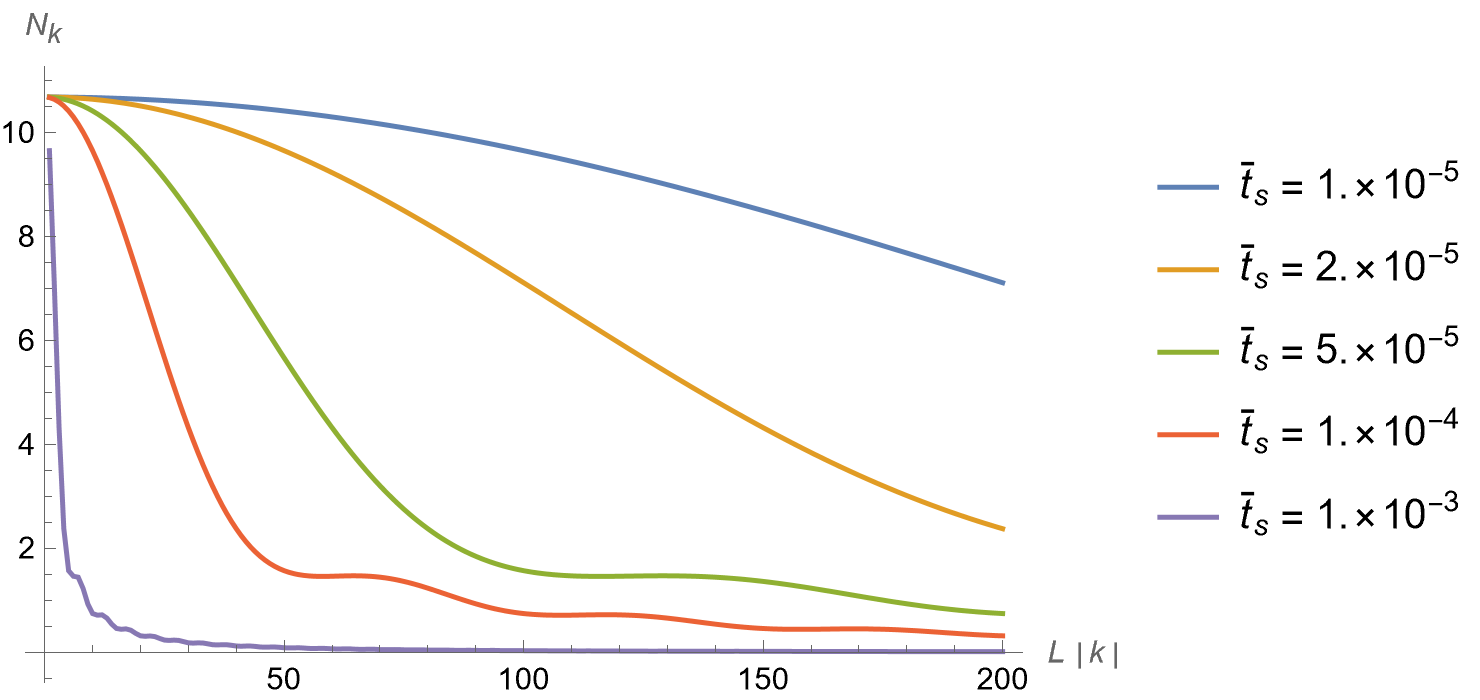
\includegraphics[width = 0.7\textwidth]{images/fig2.png}
        %     \caption{The momentum distribution when the universe stops expanding for multiple effective rates of expansion}
        %     \label{fig:finalTime}
        % \end{figure}

        % \begin{figure}[h!]
        %     \centering
        %     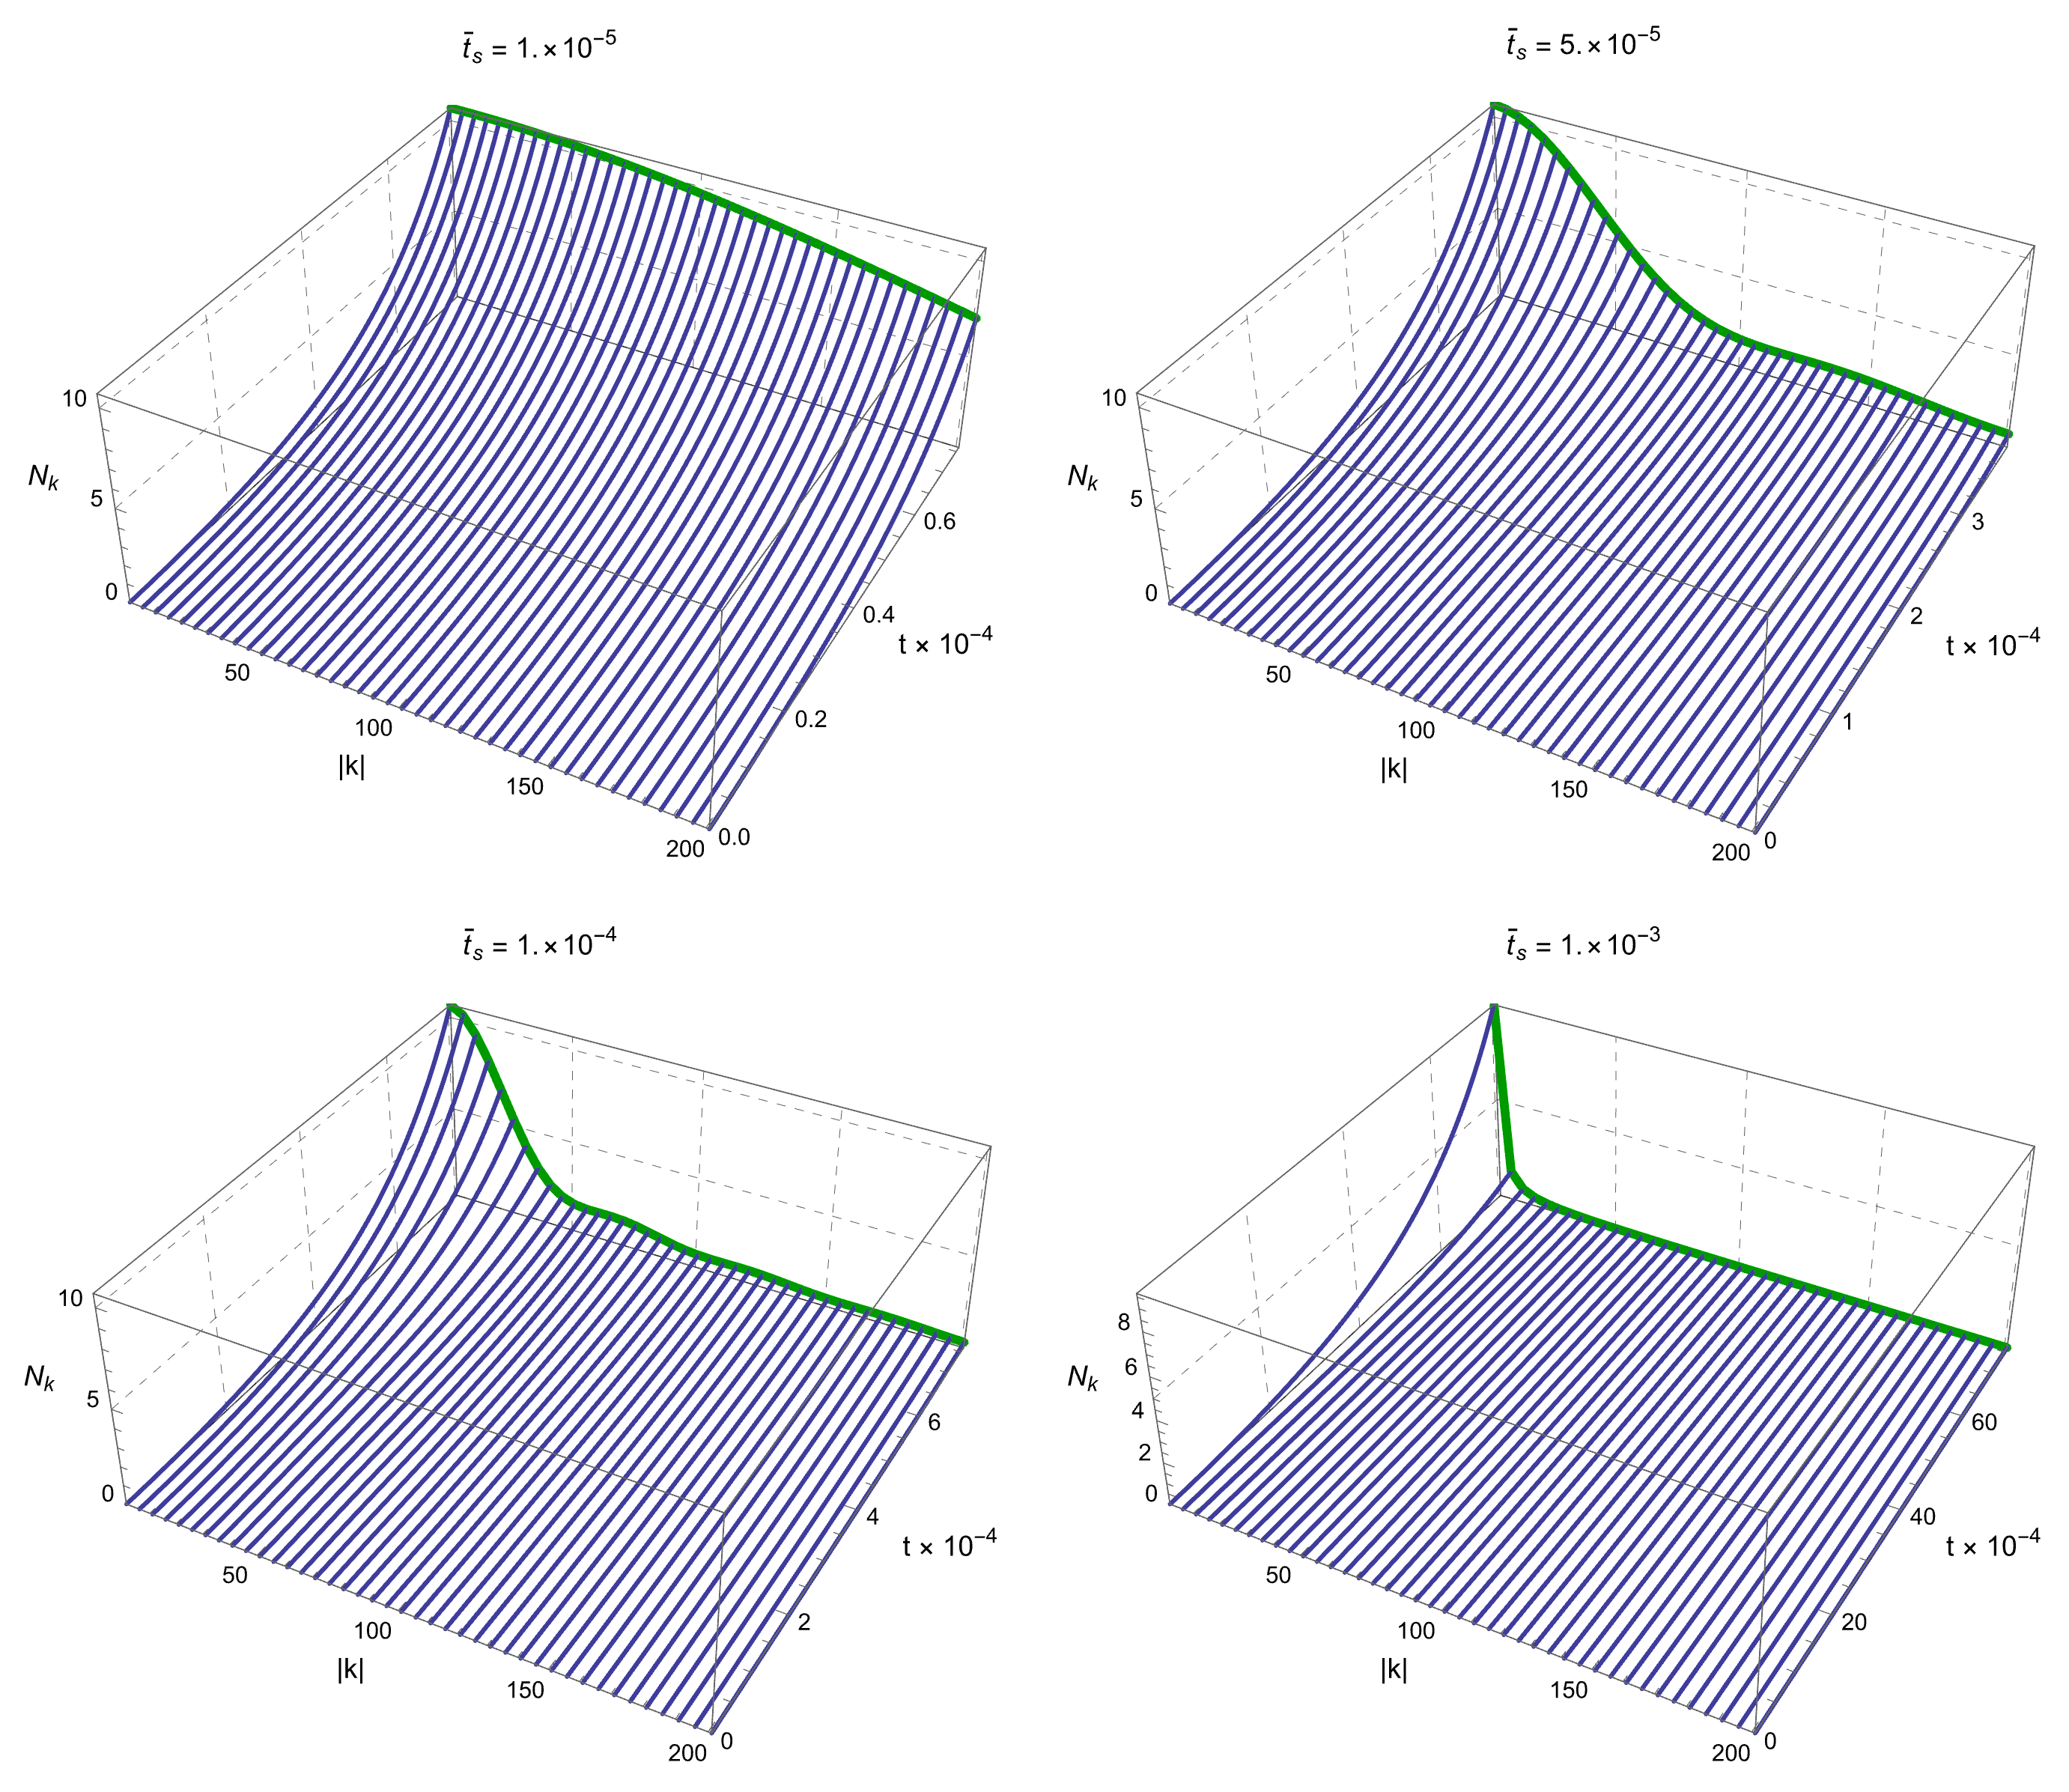
\includegraphics[width=\textwidth]{images/Analytic_Fig_4.png}
        %     \caption{Momentum distribution throughout the expansion}
        %     \label{fig:allTime}
        % \end{figure}

    % This work aims to produce several results in different facets.  From a physical perspective, we will produce the data to describe particle production in a universe undergoing a de Sitter expansion.  From an efficiency approach, we will quantitatively describe the ratio of accuracy to ``effort'' in order for future investigations to determine if using the lower-dimensional model is sufficient for their needs.  From an accessibility viewpoint, we will produce a modern, open-source, and ready-to-use computational model that is available to future investigations.

    % The particle production data will be used to show how many particles have a specific momentum at a certain time during the expansion.  Additionally, the data will be used to show how that momentum distribution changes throughout the time in which the expansion is happening.  These figures will be intended to closely follow those found in previous investigations\cite{Jain}.

    % Because previous investigations were less accurate but needed fewer computational resources and time, these results will be used to assess the efficiency of the two-dimensional model.  In other words, we aim to provide a quantitative description of whether or not the increased accuracy of the three-dimensional model warrants the extra theoretical and computational effort as compared to the two-dimensional model\cite{Jain}.

    % The final result of this work will be a packaged software that can be downloaded and used ``out of the box'', for free, by anyone that can run the program.  This level of accessibility is meant to disseminate this work to everybody that wants it.
    
\section{Upcoming Conferences}

    \begin{itemize}
        \item SOURCE - Late May
        \item APS NW - Late June
    \end{itemize}

% h) CitedliteratureorReferences(notincludedin 8-pagelimitation)
\pagebreak
\nocite{*}
\printbibliography

\end{document}
